\documentclass{article}
\usepackage{amsmath,amsfonts,amsthm,amssymb,amsopn,bm}
\usepackage[margin=.9in]{geometry}
\usepackage{graphicx}
\usepackage{url}
\usepackage[usenames,dvipsnames]{color}
\usepackage{fancyhdr}
\usepackage{multirow}
\usepackage{listings}
\usepackage{hyperref}

\definecolor{keywords}{RGB}{255,0,90}
\definecolor{comments}{RGB}{0,0,113}
\definecolor{red}{RGB}{160,0,0}
\definecolor{green}{RGB}{0,150,0}
 
\lstset{language=Python, 
        basicstyle=\ttfamily\tiny, 
        keywordstyle=\color{keywords},
        commentstyle=\color{comments},
        stringstyle=\color{red},
        showstringspaces=false}

\newcommand{\field}[1]{\mathbb{#1}}
\newcommand{\1}{\mathbf{1}}
\newcommand{\E}{\mathbb{E}} 
\newcommand{\Z}{\mathbb{Z}} 
\renewcommand{\P}{\mathbb{P}}
\newcommand{\R}{\field{R}} % real domain
% \newcommand{\C}{\field{C}} % complex domain
\newcommand{\F}{\field{F}} % functional domain
\newcommand{\T}{^{\textrm T}} % transpose
\def\diag{\text{diag}}

%% operator in linear algebra, functional analysis
\newcommand{\inner}[2]{#1\cdot #2}
\newcommand{\norm}[1]{\left\|#1\right\|}
\newcommand{\twonorm}[1]{\|#1\|_2^2}
% operator in functios, maps such as M: domain1 --> domain 2
\newcommand{\Map}[1]{\mathcal{#1}}
\renewcommand{\theenumi}{\alph{enumi}} 

\newcommand{\Perp}{\perp \! \! \! \perp}

\newcommand\independent{\protect\mathpalette{\protect\independenT}{\perp}}
\def\independenT#1#2{\mathrel{\rlap{$#1#2$}\mkern2mu{#1#2}}}
\newcommand{\vct}[1]{\boldsymbol{#1}} % vector
\newcommand{\mat}[1]{\boldsymbol{#1}} % matrix
\newcommand{\cst}[1]{\mathsf{#1}} % constant
\newcommand{\ProbOpr}[1]{\mathbb{#1}}
\newcommand{\points}[1]{\small\textcolor{magenta}{\emph{[#1 points]}} \normalsize}
\date{{}}

\setlength\parindent{0px}
\makeatletter
\DeclareUrlCommand\ULurl@@{%
  \def\UrlFont{\ttfamily\color{blue}}%
  \def\UrlLeft{\uline\bgroup}%
  \def\UrlRight{\egroup}}
\def\ULurl@#1{\hyper@linkurl{\ULurl@@{#1}}{#1}}
\DeclareRobustCommand*\ULurl{\hyper@normalise\ULurl@}
\makeatother

%\newcommand{\ind}{\mbox{$~\underline{~\parallel~}~$}}%
\newcommand{\ind}{\mbox{$\perp \kern-5.5pt \perp$}}
\newcommand{\nind}{\mbox{$\not\hspace{-4pt}\ind$}}


\begin{document}
\title{Homework \#7}
\author{\normalsize{Winter 2020, STATS 509}\\
\normalsize{Dino Bektesevic}}
\maketitle

\subsection*{Problem 1: Sampling Distributions}
A researcher plans to carry out an opinion survey regarding a yes/no question. Suppose that (unknown to the researcher) $89\%$ of people in the target population answer `yes'. We will use $1$ to denote `yes' and $0$ to denote `no'.
\begin{itemize}
    \item[a.] Let $X_1$ be the response from the first person the researcher asks. Before this person is asked, what is the distribution of $X_1$. What is $E[X_1]$ and $V(X_1)$?
\end{itemize}
The researcher plans to obtain a random sample of size $25$: $X_1,\ldots , X_{25}$. \par
(Suppose either that the researcher is sampling with replacement or that the population is so large that we may regard the samples as being taken with replacement.)
\begin{itemize} 
    \item[b.] Write down the distribution of $X_i$ for $i=1,\ldots ,25$; also write down $E[X_i]$, $V(X_i)$ and Cov$(X_i,X_j)$ for $i\neq j$.
    
    \item[c.] What is the distribution of $\bar{X}$? {\it Hint: see lecture notes.}\par
    What is the mean and variance of this distribution?
        
    \newpage
    \item[d.] Use {\tt R} or Python, replicate the experiment $10,000$ times. \par
    {\it Hint: Recall that a Bernoulli$(p)$ random variable is just a Binomial$(1,p)$ random variable; thus to obtain a sample of size $25$ from a Bernoulli$(0.89)$ random variable, one might use:\par
    {\tt p <- 0.89\par
        n <- 25\par
        x <- rbinom(n,1,p)
    }\par
    The vector {\tt x} will contain the $25$ Bernoulli$(p)$ observations, from which you can compute the sample mean. This should then be put in a loop which repeats this process, 10K times, storing the result.} Construct a histogram with the distribution of $\bar{X}$ for each sample. Does the distribution of sample means appear to be normal? Explain your answer. 
    
    \begin{center}
        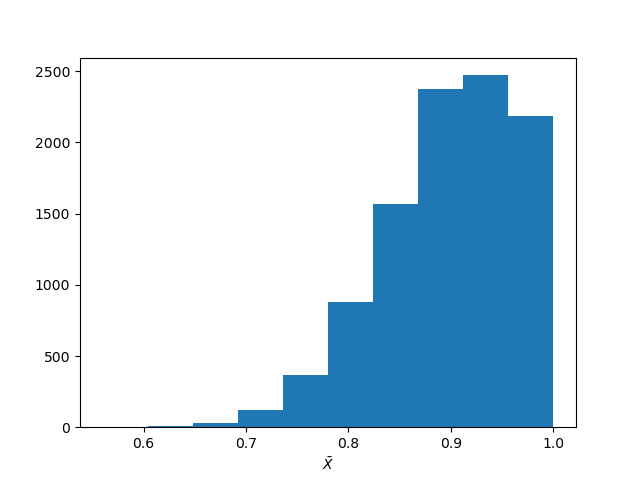
\includegraphics[width=0.5\textwidth]{STATS509/HW7/HW7Figures/Problem1.png}
    \end{center}
    
    The distribution does not look normal. 
    
    \lstinputlisting[linerange={0-22}]{STATS509/HW7/HW7Code/HW7_DinoBektesevic.py}
    
    
    \item[e.] Find the mean and variance of $\bar{X}$, based on your 10K simulations.  Does this agree with your calculation in c.?

    \lstinline[language=Python]{Mean of means: 0.8891480000000002}\newline
    \lstinline[language=Python]{Variance of means: 0.003957434095999998}

    \item[f] Compute the mean squared error of $\bar{X}$ as an estimate of the unknown proportion $\theta=0.89$ (i.e. find the squared error of the estimate, which is $(\bar{X} - \theta)^2$, in each repetition and then average over all repetitions). What do you notice? Give a simple explanation by referring to a result from the course.
    
    \lstinline[language=Python]{Mean squared error: 0.0039581600000000005}
    It is very close to the variance of means calculated above. 
    
    \end{itemize}

\newpage
\subsection*{Problem 2}
Given a sample $X_1,\ldots , X_n$  of independent Poisson$(\lambda)$ random variables, a researcher  intends to use $\bar{X}$, the sample mean, as an estimate of $\lambda$.  Suppose that $n=20$, and $\lambda=4$.
\begin{itemize}
    \item[a.] Write down the mean and variance of this distribution.
    
    \item[b.] Using {\tt R} or Python, replicate the experiment $10,000$ times. Construct a histogram with the distribution of $\bar{X}$ for each sample. Does the distribution of sample means appear to be normal? Explain your answer.
    
    \begin{center}
        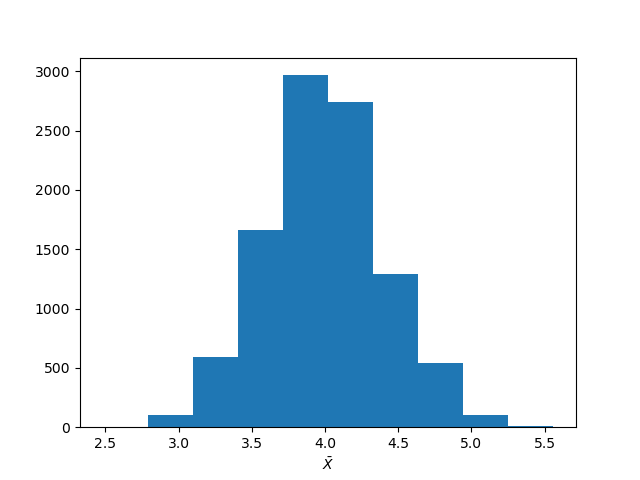
\includegraphics[width=0.5\textwidth]{STATS509/HW7/HW7Figures/Problem2.png}
    \end{center}
    
    The distribution looks normal. 
    \lstinputlisting[linerange={0-4,25-42}]{STATS509/HW7/HW7Code/HW7_DinoBektesevic.py}
    
    \item[c.] Find the mean and variance of $\bar{X}$, based on your 10K simulations. Does this agree with your calculation in a.?
    
    \lstinline[language=Python]{Mean of means: 3.9952959999999997}\newline
    \lstinline[language=Python]{Variance of means: 0.16090299238400002}
    
    \item[d.] Compute the mean squared error of $\bar{X}$ as an estimate of $\lambda$. Again what do you notice? 
    
    \lstinline[language=Python]{Mean squared error: 0.16092512}
    It is very close to the variance of means calculated above. 
\end{itemize}



\newpage
\subsection*{Problem 3: Hypothesis Tests}

Suppose that $Y_1,\ldots ,Y_n$ are i.i.d samples from a Poisson distribution with parameter $\lambda$. 
\begin{itemize}
    \item[a.] Find the log of the likelihood: $\ln f(y_1,\ldots ,y_n\,|\, \lambda)$;
    Poisson distribution is given as 
    $$ f(y_i|\lambda) = \frac{e^{-\lambda} \lambda^{y_i}}{y_i!} $$
    The likelihood can be written as:
    $$L(\lambda|y_1\hdots y_n) = \prod_{i=1}^n f(y_i|\lambda)  = \frac{\lambda^{\sum_{i=1}^n y_i} e^{-n\lambda}}{\prod_{i=1}^n y_i!}$$
    Log likelihood is then:
    $$ l(\lambda|y_1\hdots y_n) = \ln(\lambda)\sum_{i=1}^n y_i - n\lambda - \ln \prod_{i=1}^n y_i! $$ 
    
    \item[b.] By differentiating the log likelihood, find the value $\hat{\lambda}$ of $\lambda$ that maximizes the likelihood; confirm that $\hat{\lambda}$ is a maximum. The estimate  $\hat{\lambda}$  is called the {\it maximum likelihood estimator (MLE)}.
    \begin{align*}
        \frac{d}{d\lambda} l(\lambda|y_1\hdots y_n) &= \frac{d}{d\lambda}\ln(\lambda)\sum_{i=1}^n y_i - \frac{d}{d\lambda}n\lambda - \frac{d}{d\lambda}\ln \prod_{i=1}^n y_i! = 0 \\
         0 &= \frac{\sum_{i=1}^n y_i}{\hat\lambda} - n \\
         n\hat\lambda &= \sum_{i=1}^n y_i  \\
         \hat\lambda &= \frac{\sum_{i=1}^n y_i}{\lambda} \\
         \hat\lambda &= \bar y
    \end{align*}
    To confirm it's a maximum we have to take a look at the second derivative:
    \begin{align*}
        \frac{d^2}{d\lambda^2} l(\lambda|y_1\hdots y_n) &= \frac{d}{d\lambda} \frac{\sum_{i=1}^n y_i}{\lambda} \\
        &= - \frac{\sum_{i=1}^n y_i}{\lambda^2}
    \end{align*}
    Since it's always negative this is a maximum. 
\end{itemize}

Suppose that we wish to test $H_0$: $\lambda =\lambda_0$ vs. $H_1$: $\lambda \neq \lambda_0$.
\begin{itemize}
    \item[c.] Using your answer to b. write down the generalized likelihood ratio test statistic (LRT).\par
    {\it Hint: Your answer should be a function of $n$, $\lambda_0$ and $\hat{\lambda}$.}
    
    \begin{align*}
        \lambda_{lrt}(y_1\hdots y_n) &= \frac{f(y_1\hdots y_n|\lambda_0)}{\sup_{\lambda\in\R} f(y_1\hdots y_n|\lambda)} \\
        &= \frac{\lambda^{\sum_{i=1}^n y_i} e^{-n\lambda}_0}{\hat\lambda^{\sum_{i=1}^n y_i} e^{-n\hat\lambda}} \\
        &= \frac{\lambda^{\sum_{i=1}^n y_i} e^{-n\lambda}_0}{\bar y^{\sum_{i=1}^n y_i} e^{-n\bar y}} \\
        &= e^{-n(\lambda_0 - \bar y)} \left(\frac{\lambda_0}{\bar y}\right)^{n\bar y}
    \end{align*}
    
    \item[d.] Consider Bortkiewicz's Prussian Cavalry horse-kick fatality data:
    
        \begin{tabular}{l|ccccc}
        No. of fatalities & 0 & 1 & 2 & 3 & 4\\
        \hline
        No. of years & 109 & 65 & 22 & 3 & 1
        \end{tabular}
    \smallskip
    {\scriptsize The original table from Bortkiewicz's 1898 book {\it Das Gesetz der kleinen Zahlen} is: \url{https://archive.org/stream/dasgesetzderklei00bortrich#page/n66/mode/1up}}
    \smallskip
    
    Find the value of $\sum_{i=1}^{n} y_i$, and use your answer to b. to find the value of the MLE $\hat{\lambda}$.\par
    {\it Hint: The table contains data on $n=200$ observations, $y_1,\ldots ,y_{200}$, of which $109$ were $0$; there were $65$ which were $1$ and so on.}

    $$\sum_{i=1}^{200} y_i = 0\cdot 109 + 65 + 2\cdot 22 + 9 + 4 = 122$$

    So the $\bar y = \frac{122}{200} \approx 0.6$
    
    \item[e.] Use your answer to d. to find the LRT statistic for the hypothesis test with $\lambda_0=1$.\par
    
    \begin{align}
        \lambda_{lrt}(y_1\hdots y_n) &= e^{-n(\lambda_0 - \bar y)} \left(\frac{\lambda_0}{\bar y}\right)^{n\bar y} \\
        &= e^{-200(1-0.6) }\left(\frac{200}{122}\right)^{200\frac{122}{200}} \\
        &= e^{-80}\left(\frac{200}{122}\right)^{122} \\
        &= 2.79\cdot 10^{-9}
    \end{align}

    \item[f] Report the approximate p-value.\par
    {\it Hint: calculate $-2\log$(LRT), and compare to the appropriate $\chi^2$ distribution. See Lecture 10, slide 43. Recall that small values of the LRT correspond to evidence against $H_0$.}
    
\end{itemize}

\newpage
\subsection*{Problem 4}
Suppose that we are planning an experiment to test hypotheses about the mean of a population that is known to be normal with standard deviation $\sigma =4$. We wish to test the null hypothesis  $H_0: \mu = 0$ vs.~the alternative $H_A: \mu> 0$. We intend to use a likelihood ratio test with significance level $\alpha = 0.05$.
\begin{itemize}
    \item[a.] For which values of $\bar{X}$, the sample mean, will we reject the null hypothesis. Express your answer as a function of sample size, $n$.
    
    We are given that $\bar X \sim N(\mu, \sigma)$. Rewriting this to standard normal yields:
    $$Y = \frac{\sqrt{n}(\bar X - \mu)}{\sigma} \sim N(0,1)$$
    Under the null hypothesis $\mu=0$ so we relate $\alpha$ to $c$ by:
    \begin{align*}
        \alpha &= P(\bar X > c |\mu=0) \\
        &= P\left( \frac{\sqrt{n}(\bar X - \mu)}{\sigma} > \frac{\sqrt{n}(c - \mu)}{\sigma} \bigg | \mu=0\right) \\
        &= P \left(Y > \frac{\sqrt{n}(c - \mu)}{\sigma}  \bigg | \mu=0 \right) \\
        &=  1- P \left(Y < \frac{\sqrt{n}(c - \mu)}{\sigma}  \bigg | \mu=0\right) \\
        1-\alpha &= \Phi\left( \frac{\sqrt{n}(c - \mu)}{\sigma}  \bigg | \mu=0 \right) \\
        0.95 & = \Phi\left( \sqrt{n}\frac{c - \mu}{\sigma}  \bigg | \mu=0 \right) 
    \end{align*}
    The CDF of a standard normal distribution equals $0.95$ at the standard score of $1.644854$ so we can determine $c$ to be:
    \begin{align*}
        \sqrt{n}\frac{c}{4} &= 1.6644854  \\
        c &= \frac{6.579416}{\sqrt{n}}
    \end{align*}
    
    \item[b.] Suppose that we plan to obtain a sample of size $36$. The researcher thinks that if the alternative is true then perhaps $\mu = 0.3$. Calculate the power of the test to reject the null hypothesis under this particular alternative hypothesis.
    
    Equivalently to the previous problem we can start by writing:
    \begin{align*}
        1 - \beta &=  1- P \left(Y < \frac{\sqrt{n}(c - \mu)}{\sigma}  \bigg | \mu=0.3 \right) \\
        &=  1 - \Phi  \left(\frac{\sqrt{n}(c - \mu)}{\sigma}\right) \\
        &= 1- \Phi\left( \frac{\sqrt{n}(c - \mu)}{\sigma}  \bigg | \mu=0.3 \right) \\
        &= 1- \Phi\left( \frac{\sqrt{n}(\frac{6.579416}{\sqrt{n}} - \mu)}{\sigma}  \bigg | \mu=0.3 \right) \\
        &= 1- \Phi\left( \frac{6(\frac{6.579416}{6} - 0.3}{4} \right) \\
        &= 1- \Phi(1.194854 ) \\
        &= 0.116
    \end{align*}

    \item[c.] Continuing from b., the scientist who is planning the experiment wishes to have power at least $90\%$. (Thus your calculation in b. shows that more than $36$ observations are required.) Find approximately the smallest sample size at which this power can be achieved, against the specific alternative $\mu=0.3$.\par 
    {\it Hint: repeat the calculation performed in {\rm b.} at different sample sizes using trial and error: you may wish to use {\tt R} or a spreadsheet to speed up this calculation.}

   \item[d.] Suppose that the researcher obtains $200$ samples, and observes $\bar{x} = 0.65$. Compute the p-value for this hypothesis test.
   
   \begin{align*}
       p_v &= P(\bar X > \bar x | H_0) \\
       &= 1 - \Phi(\frac{\sqrt{200}(0.65 - 0)}{4} \\
       &= 0.0108
   \end{align*}
\end{itemize}


\newpage
\subsection*{Problem 5}
A researcher performs a sequence of independent experiments, up to and including the first `success', after which the researcher stops. Each experiment has the same probability $p$ of success. Let $T$ be the number of experiments  performed (including the first observed success). The researcher wishes to test the null hypothesis 
\begin{enumerate}
    \item $H_0$: $p=0.25$, 
    \item against the alternative hypothesis
    \item $H_1$:  $p>0.25$. 
\end{enumerate}
The researcher proposes to reject the null hypothesis if $T<4$.
\begin{enumerate}
    \item  What is the significance level $\alpha$ of the test proposed by the researcher?
   
    \begin{align*}
        \alpha &= P(T<4|H_0) \\
        &= P(T\leq 3 | H_0) \\
        &= \sum_{t=1}^3 p_0(1-p_0)^{t-1} \\
        &= \left(\frac{1}{4} + \frac{3}{16} + \frac{9}{64} \right) \\
        &= \frac{37}{64}
    \end{align*}
    
    \item What is the power of the researcher's test against the specific alternative hypothesis that $p=0.5$.
    
     \begin{align*}
        1- \beta &= P(T<4|H_1) \\
        &= P(T\leq 3 | H_1) \\
        &= \sum_{t=1}^3 p_1(1-p_1)^{t-1} \\
        &= \sum_{t=1}^3 0.5^t \\
        &= \left(\frac{1}{2} + \frac{1}{4} + \frac{1}{8} \right) \\
        &= \frac{7}{8}
    \end{align*}
    
    \item  Re-express the researcher's rule for rejecting the null hypothesis in terms of the likelihood ratio:
    $$ {\rm LRT} = p(t \mid p=0.25)/p(t \mid p=0.5). $$
    Specifically, find the value $\ell$ such that the researcher will reject $H_0$ $p=0.25$ in favor of $p=0.5$ if LRT$<\ell$.\par  {(Note: There will be a range of values for $\ell$ that will give the same test.)}
    
    \begin{align*}
        \Lambda (t) &= \frac{P(T=t|H_0}{P(T=t|H_1)} \\
        &= \frac{p_0(1-p_0)^{t-1}}{p_1(1-p_1)^{t-1}} \\
        &= \frac{1}{2}\left(\frac{3}{2}\right)^{t-1}
    \end{align*}
    
\end{enumerate}
{\it Hint: (For all parts) Geometric distribution!}


\newpage
\subsection*{Problem 6: Confidence Intervals}
Consider a $95\%$ confidence interval for the mean height $\mu$ in a population. Which of the following are true or false: 
\begin{enumerate}
    \item Before taking our sample,  the probability of the resulting $95\%$ confidence interval containing $\mu$ is $0.95$.
    
    True. 
    
    \item If we take a sample and compute a $95\%$ confidence interval for $\mu$ to be $[1.2,3.7]$ then $P(\mu \in [1.2,3.7]) = 0.95$.
    
    False. We can only think of $\mu$ as being random before taking a sample. Afterwards, it's just a number.
    
    \item Before taking our sample, the center of a $95\%$ confidence interval for the population mean is a random variable.
    
    True, before taking a sample the center of our interval is a random variable because it's based on the sampling a random variable.
    
    \item $95\%$ of individuals in the population have heights that lie in the $95\%$ confidence interval for $\mu$. 
    
    False. CI tells us the confidence that after drawing a random sample it's mean will lie in that range, not the other way around.
    
    \item Over hypothetical replications out of one hundred $95\%$ confidence intervals for $\mu$, on average $95$ will contain $\mu$.
    
    True.
    
    \item After obtaining our sample, the resulting confidence interval either does or does not contain $\mu$.
    
    True, we don't know if our sampled CI actually contains or doesn't contain the mean. 
\end{enumerate}




\newpage
\subsection*{Problem 7}
Goldberger Qu.~11.6 (Assume that the observations are drawn from a Normal Distribution and see Lecture 10, slide 46.)

\end{document}
